\documentclass[9pt,conference]{IEEEtran}
\IEEEoverridecommandlockouts
\usepackage{cite}
\usepackage{amsmath,amssymb,amsfonts}
\usepackage{algorithmic}
\usepackage{graphicx}
\usepackage{textcomp}
\usepackage{xcolor}
\usepackage{array}
\usepackage{multirow}
\usepackage{hyperref}
\usepackage{makecell}
\usepackage{diagbox}
\usepackage{tikz}
\usepackage{booktabs}
\usepackage{threeparttable}
\def\BibTeX{{\rm B\kern-.05em{\sc i\kern-.025em b}\kern-.08em
    T\kern-.1667em\lower.7ex\hbox{E}\kern-.125emX}}
\begin{document}

\title{Post-Layout Evaluation and Tapeout of a Streamlined Domain-Specific VLIW Architecture with Custom RISC-V Extensions for Wireless Baseband\\
% \thanks{funding agency etc.}
}

% \author{
%   Rui Hong\textsuperscript{1}, Man Dai\textsuperscript{1}, Lin Liu\textsuperscript{1}, 
%   Pan Liu\textsuperscript{2}, Yimin Du\textsuperscript{1}, Shuoming Zhang\textsuperscript{1},
%   Jinglin Shi\textsuperscript{1,*} \\[1pt]
%   \normalsize State Key Lab of Processors, Institute of Computing Technology, CAS, Beijing 100190, China \\[1pt]
%   \normalsize University of Chinese Academy of Sciences \\[1pt]
%   \normalsize \textsuperscript{1}\{hongrui, daiman2019, liulin11, duyimin, zhangshuoming21s, sjl\}@ict.ac.cn \\
%   \normalsize \textsuperscript{2}liupan241@mails.ucas.ac.cn
% }

\maketitle

\begin{abstract}
This paper presents a streamlined domain-specific VLIW architecture with custom RISC-V ISA extensions tailored for wireless baseband signal processing, which achieves a well-balanced trade-off between programmability and hardware efficiency through hardware-software co-design. The design has completed full sign-off backend implementation in TSMC 22 nm ULL technology at 800 MHz, and has been integrated and taped out in a three-core SparkLink SLB 2.0 baseband SoC. Its core area is less than half that of state-of-the-art 16 nm commercial DSPs, with strong dynamic power efficiency. All system-level latency and real-time requirements are fully satisfied under peak workloads.
\end{abstract}

\section{Introduction}
Wireless communication systems now must support a diverse range of standards spanning short-range connectivity to cellular and satellite networks, imposing growing demands for both efficiency and flexibility on baseband chip design. Application Specific Integrated Circuits (ASICs) deliver high power efficiency for fixed workloads such as channel coding \cite{shao2019survey}, but their limited scalability shortens product lifecycles and raises iteration costs, especially when accommodating multiple evolving standards. This has driven continuous research into more flexible yet efficient digital baseband processing architectures.

Software Defined Radio (SDR) has been widely explored as a flexible alternative, with extensive work on algorithm mapping and optimization onto CPUs, GPUs, DSPs and FPGAs \cite{sinha2016software, akeela2018software}. Prior work has also proposed various specialized processing architectures\cite{anjum2011state}, including DSP-style designs \cite{liu2009bridging, moudgill2008sandblaster, highefficient, ziyuan2013100} and many-core/dataflow architectures such as GPU-like/CGRA-like \cite{lin2007soda, woh2008soda, bougard2008coarse, wu2023alleviating}. While these solutions greatly improve flexibility over ASICs, most commercial processor IPs follow a general-purpose design philosophy that introduces substantial architectural redundancy. This is primarily because maximizing commercial interests inherently inclines these IPs towards supporting a wide array of application scenarios. For example, general-purpose DSPs must compromise across wired communication, audio/video codec and even AI workloads, leaving many instructions underutilized in specific wireless scenarios, which degrades energy efficiency and adds licensing overhead. In \cite{amor2021risc} the author analyzed that some commercial DSP ISAs have a large instruction count and many are of little practical use in RF algorithms. And \cite{amor2019software} pointed out that ARM Cortex-M is a bit too redundant for IoT applications. Many-core and CGRA-like designs, meanwhile, often suffer from low compute resource utilization, making it challenging to optimize area and power simultaneously. So it is indeed a better option to design own ISA and new domain-specific architecture, which requires profound design experience.

The open, royalty-free RISC-V ISA provides a promising foundation for domain-specific customization, with well-defined ISA encoding rules and strong extensibility \cite{cui2023risc}. Developers can make their own extensions that are different from official ones according to the needs of their own application fields, getting much better overall results than general purpose IPs. Existing work has explored standard RISC-V extensions for communication workloads \cite{razilov2022communications, li2023portable}, as well as custom ISA extensions for baseband processing \cite{amor2021risc, melo2016oolong}, low-power DSP operations \cite{gautschi2017near}, hardware security \cite{palmiero2018design}, bit-level operations like channel-coding \cite{tourres2021extended}, and upper-layer protocol optimization \cite{andri2020extending, paulin2021rnn}.

While VLIW architectures have seen limited adoption in general-purpose computing due to their workload-specific nature, their streamlined hardware logic makes them well suited for domain-specific computing, where targeted optimization can deliver high performance with low area and power overhead. This paper presents a domain-specific VLIW architecture with custom RISC-V ISA extensions, tailored for wireless baseband signal processing. The main contributions of this work are:

\begin{enumerate}
    \item We analyze common computational paradigms across wireless signal processing flows and derive a set of fundamental operators, leveraging the observation that baseband computation patterns remain largely consistent across evolving communication standards.
    \item We propose a streamlined domain-specific VLIW architecture and dedicated co-processor tailored for wireless baseband processing, with a custom RISC-V ISA extension and an associated LLVM-based compiler featuring a hybrid instruction scheduling algorithm to achieve superior software optimization.
    \item We fully validate the design in a production-grade SparkLink \cite{gao2023sparklink} SLB (SparkLink Basic) 2.0 baseband SoC. The design has completed full sign-off backend implementation in TSMC 22 nm ULL technology and been taped out in a three-core configuration. Post-layout results show the core area is less than half that of state-of-the-art 16 nm commercial DSPs, with favorable dynamic power efficiency, and all system-level latency and real-time requirements of SLB 2.0 are fully satisfied under peak workloads.
\end{enumerate}

\section{Background \& Motivation}

\subsection{Common Computational Paradigms in Wireless Communication Signal Processing}

Despite the diversity of modern wireless communication standards, their physical layer processing flows share fundamentally consistent computational paradigms. Transmitter-side operations including encoding, modulation, resource mapping and waveform generation, as well as receiver-side procedures such as synchronization, channel estimation, equalization, demodulation and decoding, can all be decomposed into a set of reusable elementary operators.

For example, sequence cross-correlation for synchronization, cyclic prefix autocorrelation for timing detection, and FIR filtering all belong to the same category of multiply-accumulate intensive sequence operations. Channel estimation and equalization rely on common vector arithmetic and matrix operations, while FFT/IFFT transforms share unified butterfly computation patterns. This cross-standard and cross-module computational commonality forms the foundation of domain-specific architecture design: by tailoring hardware to these core operators, it is possible to retain programming flexibility while eliminating the functional redundancy inherent in general-purpose cores, thus achieving superior area and power efficiency.

Through a comprehensive analysis of physical layer processing flows across multiple mainstream wireless standards, we summarize the core common operators and their corresponding typical physical-layer modules, as shown in Table \autoref{tab:operator}. These operators define the core direction of the ISA design and functional unit configuration in the proposed architecture.

\begin{table}
\centering
\caption{Common Operators of Wireless Communication Signal Processing}
\label{tab:operator}
\begin{tabular}{|>{\raggedright\arraybackslash}p{0.35\linewidth}|>{\raggedright\arraybackslash}p{0.55\linewidth}|}
\hline
\multicolumn{1}{|>{\centering\arraybackslash}p{0.35\linewidth}|}{\textbf{Operators}} & 
\multicolumn{1}{>{\centering\arraybackslash}p{0.55\linewidth}|}{\textbf{Typical Physical-layer Modules}} \\ \hline
Maximum & Finding peak values \\ \hline
Sequence Correlation/Filtering/Convolution & FIR filtering and Synchronization \\ \hline
Sequence Multiplication & Frequency Compensation and Channel Estimation \\ \hline
Divide & Channel Equalization \\ \hline
Euler Formula & Sequence Generation and Trigonometric Function \\ \hline
Data Extraction & Resource Mapping and Resource De-mapping \\ \hline
Baseband Modulation & BPSK, QPSK, 16QAM, 64QAM, 256QAM, 1024QAM \\ \hline
Butterfly Operation & FFT, IFFT, DFT, IDFT \\ \hline
Sort & Channel Parameter Analysis \\ \hline
Remainder & Sequence Generation and Parameter Calculation \\ \hline
Exponentiation & Channel Measurement \\ \hline
Logarithmic Operation & Channel Measurement \\ \hline
Matrix Multiplication & Channel Equalization \\ \hline
Adjoint Matrix & Channel Equalization \\ \hline
Saturation & Accuracy Preservation during the calculation process \\ \hline
\end{tabular}
\end{table}

\subsection{SLB 2.0 : The New SparkLink Evolution}

SparkLink SLB is an emerging short-range broadband communication standard undergoing rapid evolution. Compared to other short-range communication standards like Wi-Fi, it is architected with inherent advantages in lower latency and lower power consumption at the protocol design level, while simultaneously offering superior reliability, security, connection density, and transmission rates.

In terms of physical layer data processing, the computational paradigm of SparkLink SLB remains within the aforementioned categories. However, compared to NR and LTE, processing signals of the same bandwidth in SLB demands greater computational capability, primarily due to:

\begin{enumerate}
    \item Shorter symbol duration.
    \item Reduced pipeline stages for data processing.
    \item Finer granularity of control and scheduling.
\end{enumerate}

SparkLink SLB 2.0, released by the International SparkLink Alliance in March 2025, introduces further advanced technical features, including:

\begin{enumerate}
    \item Multi-domain synchronization and 3D-FISA technology, providing enhanced anti-interference capabilities.
    \item More flexible frame types and configuration parameters, enabling broader coverage.
    \item Centralized scheduling, optimizing low-power performance.
    \item A shorter frame structure, facilitating lower latency.
\end{enumerate}

Due to substantial technical advancements, SLB 2.0 is not backward-compatible with SLB 1.0. Consequently, standards like the SparkLink SLB present significant new challenges for wireless baseband processing architectures. On one hand, the architecture must maintain flexibility to adapt to continuously evolving standards. On the other hand, it must deliver higher processing performance while achieving lower power consumption and a smaller silicon area. Traditional general-purpose architectures struggle to meet these demands. For instance, many general-purpose DSP IP cores often feature over 300 or even more instruction types, many of which are not specifically designed for wireless communication. The redundancy in the functionality and logic of these instructions leads to increased area and power overhead. This underscores the critical need for a new software-defined domain-specific architecture explicitly designed for the computational paradigms of wireless baseband processing.

\section{VLIW Architecture Design}

\subsection{ISA Design Methodology}
We base our ISA design on the standard RV32 fixed 32-bit encoding framework, preserving the core field alignment to maintain lightweight and efficient decode logic of processor front-end. Targeted at the VLIW architecture and domain-specific wireless baseband workloads, we introduce 2 key modifications to the baseline encoding, as illustrated in \autoref{fig:key-ISA-modifications}.

\begin{figure}
    \centering
    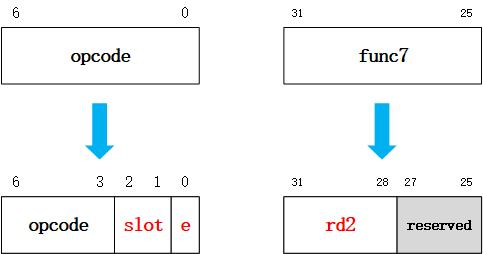
\includegraphics[width=1\linewidth]{Figs/key ISA modification.jpg}
    \caption{Key ISA Encoding Customizations}
    \label{fig:key-ISA-modifications}
\end{figure}

First, the least significant bit (LSB) is defined as the end-of-group flag. When cleared, the current instruction is concatenated with the following one to form a variable-length (up to 4) VLIW bundle; when set, it marks the last instruction in the bundle. This variable-length VLIW scheme eliminates most of the mandatory NOP padding required by fixed-length VLIW designs, effectively reducing code size, lowering instruction fetch overhead, and conserving on-chip program memory footprint. Bits 1–2 encode the VLIW slot index, supporting 4 parallel issue slots. Combined with the end-of-group flag of bit 0, this 3-bit prefix enables the decode stage to fully resolve VLIW bundle boundaries and determine the dispatch destination of each instruction using only the first three bits of the instruction word, resulting in very lightweight decode and dispatch logic with negligible timing overhead. Second, to accommodate full-precision computation patterns in wireless baseband processing, we extend a subset of R-type instructions with a second destination register field. The upper 4 bits (bits 28–31) of the original funct7 field are repurposed as the \textit{rd2} operand, while bits 25–27 remain reserved. This design allows a single instruction to output two register results, which is highly beneficial for operations such as wide multiply-accumulate, matrix multiplication, dot product, and combined division/remainder calculation. Without dual destinations, these operations would require two separate instructions to output the full-width result, degrading throughput and increasing code size. Through the aforementioned modifications, we have established a customized base instruction encoding tailored to our VLIW design. All other instructions are designed in compliance with this fundamental encoding scheme, maintaining the simplicity and efficiency of the VLIW front-end logic.

We also extend the immediate fields of B-type and J-type instructions by 1 bit. Since all instructions are 32-bit fixed length, all jump targets are 32-bit aligned. By reusing this redundant alignment bit, the branch offset range of B-type instructions and the jump range of J-type instructions are both expanded, improving control flow flexibility for potential large baseband program binaries. We further organize all domain-specific instructions by the type of the destination register in the opcode field and by source operand type in the funct3 field. This classification allows the decode unit to identify the register file type and VLIW slot at an early pipeline stage, simplifying forwarding logic and hazard detection.

It is worth noting that in standard RISC-V ISA encoding, the first 2-bit prefix are always 11 for RV32 32-bit instructions and those with 2-bit prefix 00, 01, 10 are used for the optional standard RISC-V C (compressed) extension \cite{waterman2019risc}. To simplify the pipeline front-end and enlarge available encoding space, we do not support the standard C extension. The corresponding encoding space is repurposed for VLIW and domain-specific features, quadrupling the usable opcode space within the fixed 32-bit format.

Regarding SIMD vector processing, we adopt a custom domain-specific extension instead of the standard RISC-V V or P extensions. As mentioned above, core baseband operators such as dedicated modulation, specialized matrix operations, and FFT computation are not covered by standard vector extensions, requiring custom ISA extensions anyway. Meanwhile, general-purpose vector features such as vector unit-stride and dynamic vector length configuration introduce unnecessary hardware complexity and redundancy for our targeted workloads. Our custom extension is tightly coupled with the identified common baseband operators, achieving higher efficiency with a much simpler microarchitecture.

Although this non-standard encoding breaks compatibility with off-the-shelf RISC-V toolchains, we prioritize domain-specific efficiency over standard compatibility given the closed nature of baseband computing scenarios. Compiler support and optimization will be explained later in subsection.

\subsection{Co-Processor Design}
Built upon the proposed ISA extension, we design a 4-way domain-specific VLIW co-processor optimized for wireless baseband processing. Its overall architecture is depicted in \autoref{fig:arch}. Each basic instruction length is 32-bit, and up to 4 basic instructions combine to form a 128-bit long instruction, which is dispatched to 4-issue VLIW slots. The co-processor implements a 10-stage pipeline to balance critical path timing and pipeline throughput. Certain complex vector operations and application-specific functions such as CORDIC exhibit longer execution cycle latencies, so they are implemented as multi-cycle functional units (MCFU), which operate independently without stalling the main pipeline.

\begin{figure}
    \centering
    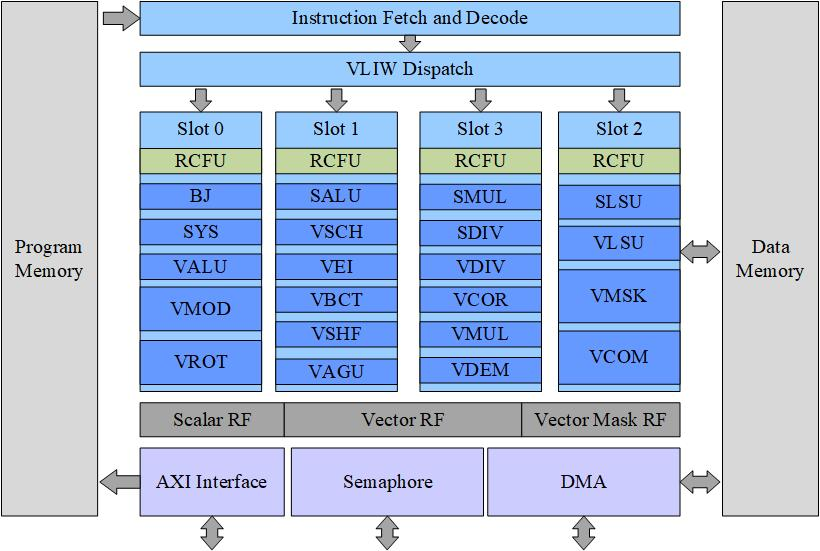
\includegraphics[width=1\linewidth]{Figs/Architecture Block Diagram.jpg}
    \caption{Core Architecture Block Diagram}
    \label{fig:arch}
\end{figure}

The register file organization is tailored for wireless baseband processing. It includes 16 32-bit general-purpose scalar registers, 16 640-bit vector registers, and 4 32-bit vector mask registers. Each 640-bit vector register holds 16 40-bit elements, illustrated in \autoref{fig:simd}, where each element consists of high 16-bit, low 16-bit, and 2 4-bit guard segments. These guard bits effectively prevent precision loss caused by overflow during iterative baseband computations, such as successive filtering and channel equalization, while maintaining flexible data width.

\begin{figure}
    \centering
    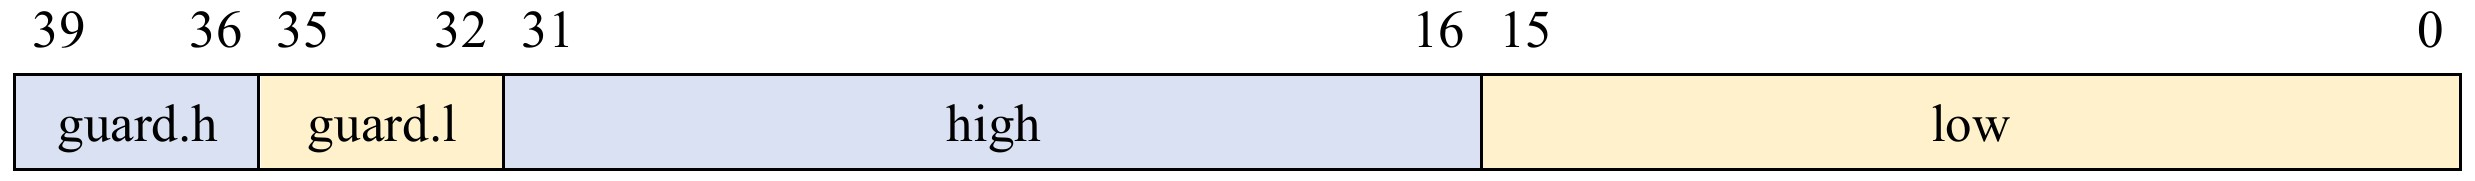
\includegraphics[width=1\linewidth]{Figs/Basic SIMD Vector Element.jpg}
    \caption{Basic SIMD Vector Element Structure}
    \label{fig:simd}
\end{figure}

Functional units are partitioned across the 4 VLIW slots according to their functionality and execution frequency, as detailed in \autoref{tab:fu}. A key optimization is the \textit{Replicated Common Functional Units (RCFU)}, which are instantiated in all 4 slots. RCFU cover the most frequently used basic scalar arithmetic, logic, and shift operations. Since these units have a very small silicon footprint, replicating them across all slots introduces negligible area overhead while significantly relaxing instruction scheduling constraints and improving achievable instruction-level parallelism (ILP).

Slot 0 handles program control operations and basic vector arithmetic. Slot 1 integrates scalar arithmetic and auxiliary vector operations. Slot 2 is dedicated to all load/store memory access operations. Slot 3 implements computation-intensive complex operations. The corresponding instructions for functional unit BJ, SYS, SALU, SLSU are basically from RV32I, and instructions for SMUL, SDIV are from RV32M. Note that in \autoref{fig:arch}, slots 2 and 3 are swapped for clearer illustration of the datapath between slot 2 and the data memory. Our workload analysis shows that operations assigned to the same slot have low concurrency probability in typical baseband flows, which maximizes ILP utilization under the heterogeneous slot organization. Additionally, by assigning all load/store instructions to a single VLIW slot, we simplify the data memory interface design, thereby reducingoverall area.

\begin{table}[htbp]
\centering
\caption{Functional Units and Descriptions}
\label{tab:fu}
\begin{tabular}{|>{\centering\arraybackslash}p{0.25\linewidth}|>{\centering\arraybackslash}p{0.15\linewidth}|>{\raggedright\arraybackslash}p{0.45\linewidth}|}
\hline
\textbf{VLIW Slot} & \textbf{Functional Unit} & \multicolumn{1}{>{\centering\arraybackslash}p{0.45\linewidth}|}{\textbf{Description}} \\
\hline
\multirow{6}{*}{\makecell[c]{0 \\ (Program Control \\ \& Simple Vector)}} 
& RCFU & Replicated Common Functional Unit (available in all slots)\\
\cline{2-3}
& BJ & Branch and Jump (from RV32I) \\
\cline{2-3}
& SYS & System control (wfi only, from RV32I) \\
\cline{2-3}
& VALU & Vector Arithmetic and Logic Operations \\
\cline{2-3}
& VMOD & Vector Modulation \\
\cline{2-3}
& VROT & Vector Rotate \\
\hline
\multirow{7}{*}{\makecell[c]{1 \\ (Scalar \& \\ Simple Vector)}}
& RCFU & Replicated Common Functional Unit (available in all slots)\\
\cline{2-3}
& SALU & Scalar Arithmetic and Logic Operations (from RV32I) \\
\cline{2-3}
& VSCH & Vector Search \\
\cline{2-3}
& VEI & Vector Extract and Insert \\
\cline{2-3}
& VBCT & Vector Bit Count \\
\cline{2-3}
& VSHF & Vector Shuffle \\
\cline{2-3}
& VAGU & Vector Address Operations \\
\hline
\multirow{5}{*}{\makecell[c]{2 \\ (Load and Store \\ related)}}
& RCFU & Replicated Common Functional Unit (available in all slots)\\
\cline{2-3}
& SLSU & Scalar Load and Store (from RV32I) \\
\cline{2-3}
& VLSU & Vector Load and Store \\
\cline{2-3}
& VMSK & Vector Mask / Predicate \\
\cline{2-3}
& VCOM & Vector Compare \\
\hline
\multirow{7}{*}{\makecell[c]{3 \\ (Complex \\ Operations)}}
& RCFU & Replicated Common Functional Unit (available in all slots)\\
\cline{2-3}
& SMUL & Scalar Multiply (from RV32M) \\
\cline{2-3}
& SDIV & Scalar Division (from RV32M) \\
\cline{2-3}
& VDIV & Vector Division \\
\cline{2-3}
& VCOR & Vector CORDIC \\
\cline{2-3}
& VMUL & Vector Multiply and Multiply-Accumulate \\
\cline{2-3}
& VDEM & Vector Demodulation \\
\hline
\end{tabular}
\end{table}

At the architecture level, the co-processor exploits both ILP via VLIW and data-level parallelism (DLP) via wide SIMD vectors. As a static multi-issue architecture, VLIW relies on the compiler/software to schedule parallel instructions, avoiding complex dynamic dependency check logic and reducing hardware overhead. When the compiler cannot fill all slots with useful instructions, the hardware automatically inserts NOPs into idle slots, eliminating the need for explicit padding in program code and further reducing code size. The combination of VLIW ILP and custom SIMD DLP delivers high throughput for baseband workloads while maintaining a streamlined and area-efficient hardware design. The hardware-software co-design principle permeates the entire design process of this domain-specific VLIW architecture, with the overarching goal of delivering a well-balanced and highly efficient overall system for wireless baseband processing.

The co-processor also integrates a complete subsystem interface, including an AXI bus interface, configurable tightly coupled memory (TCM) for program and data, a DMA engine for efficient bulk data transfer, and a lightweight semaphore unit for external input signals and events.

\subsection{Compiler Support and Instruction Scheduling Optimization}

To fully unleash the performance potential of the proposed domain-specific VLIW architecture, a tailored compiler toolchain is indispensable, as instruction-level parallelism in VLIW designs is entirely extracted and scheduled at compile time. We build our compiler backend upon the LLVM framework, with full support for our custom RISC-V VLIW encoding semantics, including variable-length instruction bundles marked by end-of-group bits and four-slot VLIW dispatch rules. Unlike fixed-length VLIW schemes that mandate nop padding for underutilized slots, our variable-length encoding eliminates redundant filler instructions, which effectively reduces generated code size, lowers instruction fetch overhead, and conserves on-chip instruction memory footprint.

At the core of our compiler optimization is a hybrid instruction scheduling algorithm that addresses the long-standing trade-off between scheduling optimality and compilation complexity. For our heterogeneous functional unit organization, where each VLIW slot supports only a dedicated subset of instruction types, conventional list scheduling often suffers from suboptimal resource utilization, while exhaustive integer linear programming scheduling delivers optimal parallelism extraction but incurs prohibitive compilation overhead. Our hybrid approach introduces a lightweight IPC theoretical upper-bound model derived from data-flow analysis, which captures both instruction dependency constraints and hardware resource limitations. The compiler first applies fast list scheduling across all scheduling regions; only regions where list scheduling fails to reach the theoretical performance bound are further refined with integer linear programming scheduling. This strategy achieves near-optimal scheduling quality while substantially reducing compilation time, making it well suited for production-grade baseband software development.

Beyond static scheduling optimization, we identify AI-driven compiler co-design as a promising future direction for this work. While our current manually tuned scheduling framework already delivers strong efficiency, the rapid evolution of wireless communication standards and continuous architecture extensions create growing pressure for faster toolchain iteration. Inspired by advances in AI-driven software/toolchain development\cite{liao2026kernelevolve}\cite{ye2026cake}, we argue that domain-specific VLIW compilation is highly amenable to AI automation, thanks to its well-defined hardware resource contracts and structured scheduling constraints. We are exploring an agent-augmented compiler paradigm for our VLIW architecture, where structured performance diagnostics and hardware conformance feedback are used to automate scheduling rule refinement, custom instruction lowering, and cross-module performance tuning. This direction is expected to drastically reduce the development cycle of domain-specific VLIW toolchains and unlock deeper architectural optimization opportunities.

\section{Implementation and Evaluation}

\subsection{SparkLink SLB Baseband SoC Topview}

Based on the proposed co-processor (Co-Pro for short in the following text), we have developed a full baseband SoC with 3 Co-Pros for the SparkLink SLB wideband standard. As previously mentioned, the significant enhancements in SparkLink SLB 2.0 result in non-backward compatibility with SLB 1.0; a foreseeable trend is the continuous evolution of further protocol iterations. Evidently, for communication standards undergoing continuous evolution like SparkLink, a fully fixed-function ASIC accelerator approach is nearly infeasible. The accelerator or chip itself must incorporate programmability to adapt to the evolving communication standard and provide sufficient performance or microarchitectural flexibility for future rapid iterations. This constitutes the fundamental rationale behind our design of the domain-specific VLIW architecture presented in this work.

The architecture overview of the baseband SoC is shown in \autoref{fig:soc}. The SoC features a complete physical layer (PHY) subsystem and protocol stack (PS) subsystem designed for the SparkLink SLB protocol. The PHY subsystem integrates 3 Co-Pros designed to handle most symbol-level computations in data flow and key L1 control tasks. The system supports a maximum bandwidth of 80M@2T2R, achieving an actual peak throughput of 800Mbps.

\begin{figure}
    \centering
    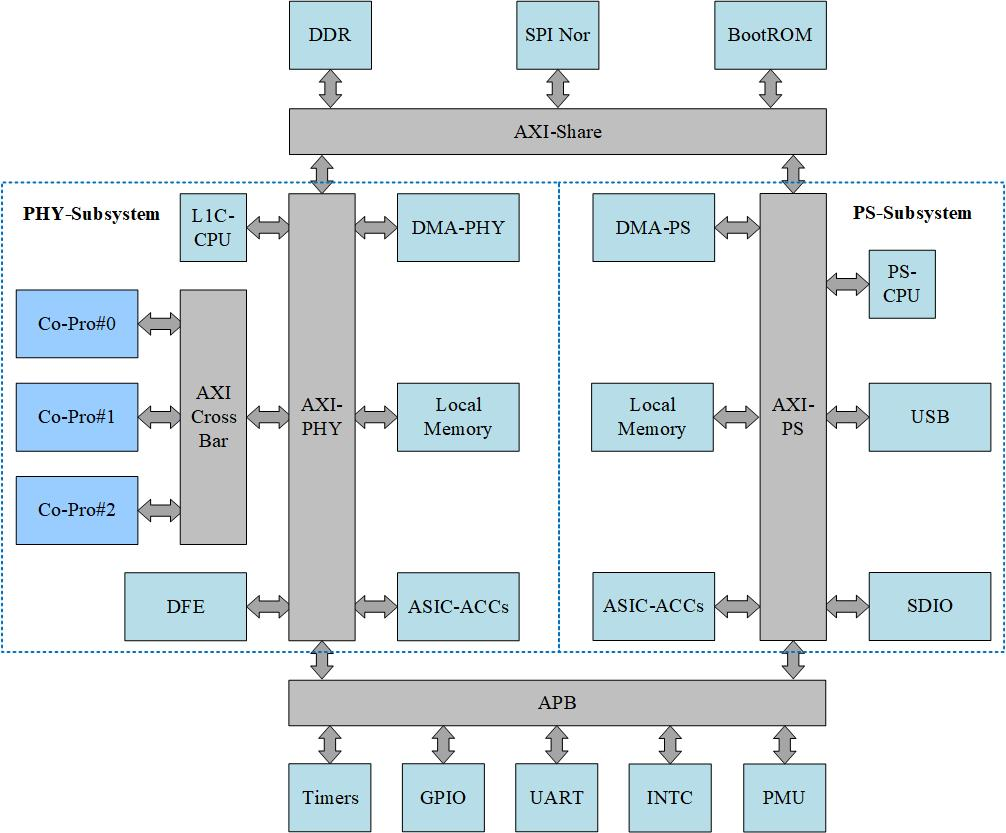
\includegraphics[width=1\linewidth]{Figs/Overview of the CoPro-based baseband SoC for SparkLink SLB.jpg}
    \caption{Overview of the Co-Pro-based baseband SoC for SparkLink SLB}
    \label{fig:soc}
\end{figure}

\subsection{Physical Implementation and Validation}

\begin{table}
    \centering
    \caption{Post-Layout Key Metrics Comparison}
    \label{tab:metrics}
    \begin{threeparttable}
    \renewcommand{\arraystretch}{1.4}
    \setlength{\extrarowheight}{2pt}
    \begin{tabular}{|>{\centering\arraybackslash}m{2.2cm}|>{\centering\arraybackslash}m{1.6cm}|>{\centering\arraybackslash}m{1.6cm}|>{\centering\arraybackslash}m{1.6cm}|}
        \hline
        \textbf{} & \textbf{Proposed Co-Pro} & \textbf{CEVA XC12} & \textbf{Tensilica B20} \\
        \hline
        \textbf{Technology Node}& TSMC 22 nm ULL& TSMC 16 nm FCLL& TSMC 16 nm \\
        \hline
        \textbf{Operating Frequency}& 800 MHz& 600 MHz & 1.1 GHz \\
        \hline
        \textbf{Core STD Cell Area}& 0.98 mm\textsuperscript{2}& 2.08 mm\textsuperscript{2} & 0.966 mm\textsuperscript{2} \\
        \hline
        \textbf{Core Dynamic Power}& 573.4 mW& 1044 mW& 786.5 mW\\\hline
    \end{tabular}
    \begin{tablenotes}[flushleft]
        \scriptsize
        \item All results are extracted from full sign-off post-place-and-route backend flows to ensure a consistent comparison basis.
        \item Proposed Co-Pro: dynamic power measured on fft\_256 workload, TT process corner, 0.90\,V supply, 85\,°C.
        \item CEVA XC12: dynamic power measured on fft\_2048 workload, typical TT corner, 0.8\,V supply, 25\,°C.
        \item Tensilica B20: dynamic power measured on fixed-point vector MAC workload, typical TT corner, 0.8\,V supply, 25\,°C.
    \end{tablenotes}
    \end{threeparttable}
\end{table}

The Co-Pro and the baseband SoC has completed full sign-off backend implementation with final GDSII generated for tapeout. All area and power metrics presented here are extracted from post-place-and-route results. For a fair and consistent comparison, all reference commercial DSP IP data are also sourced from official vendor-released full post-layout implementation reports.

\autoref{tab:metrics} summarizes the key physical implementation metrics against two state-of-the-art general-purpose DSP IPs. Fabricated in TSMC 22 nm ULL technology, the Co-Pro runs at 800 MHz with a core STD cell area of 0.98 mm². Despite adopting a more mature and less area-efficient technology node, our design achieves strong area compactness: its core area is less than half that of the 16 nm CEVA XC12, and is comparable to the 16 nm Tensilica B20. This efficiency gain comes from the streamlined domain-specific architecture, which eliminates redundant functional units and rarely used instruction logic inherent to general-purpose DSP designs.

For power evaluation, we focus the comparison on core dynamic power. Leakage power is strongly dominated by technology node, operating voltage, and junction temperature, and thus cannot directly reflect the inherent efficiency of architectural design. For continuous wireless baseband signal processing workloads, dynamic power accounts for the dominant share of total power consumption, making it the most practically relevant metric for system deployment.

Measured on a representative FFT baseband workload at typical process conditions, the core dynamic power of our design is 573.4 mW at 800 MHz. Even with the disadvantage of a older technology node, the proposed architecture delivers favorable power efficiency relative to baseband processing throughput compared with the two state-of-the-art commercial DSP IPs implemented on the more advanced 16 nm node. These post-layout results confirm the effectiveness of the domain-specific VLIW design in optimizing area and power for wireless baseband scenarios.

\subsection{Software and System Evaluation}

We conduct comprehensive evaluations across symbol, link, and system levels in a production-grade SparkLink SLB 2.0 baseband system. All tests are performed under the peak protocol configuration of 80 MHz bandwidth with 2T2R and 4 concurrent users, the most computation-intensive scenario defined in SLB 2.0. The three Co-Pros follow a heterogeneous partitioning scheme: Co-Pro\#0 performs L1 control, task scheduling, and data flow orchestration, while Co-Pro\#1 and Co-Pro\#2 execute physical-layer computation kernels including synchronization, channel estimation, equalization, and demodulation.

\begin{table}[htbp]
    \centering
    \caption{Symbol-Level Real-Time Performance}
    \label{tab:symbol_perf}
    \begin{threeparttable}
    \renewcommand{\arraystretch}{1.3}
    \footnotesize
    \setlength{\tabcolsep}{4pt}
    \begin{tabular}{|>{\raggedright\arraybackslash}m{2.8cm}|c|c|c|}
        \hline
        \textbf{Processing Module} & \textbf{Measured ($\mu\mathrm{s}$)} & \textbf{Budget ($\mu\mathrm{s}$)} & \textbf{Margin (\%)} \\
        \hline
        \multicolumn{4}{|c|}{\textit{Co-Pro\#0: Control \& Scheduling Core}} \\
        \hline
        Tx: worst case of 49 symbols & 8.923 & 8.928 & 0.06 \\
        Rx: single-user peak & 6.979 & 8.928 & 21.83 \\
        Rx: 4-user DATA peak & 8.710 & 8.928 & 2.44 \\
        \hline
        \multicolumn{4}{|c|}{\textit{Co-Pro\#1/2: Physical-Layer Computation Cores}} \\
        \hline
        Initial synchronization & 18.696 & 22.50 & 16.91 \\
        Tracking synchronization & 9.404 & 16.055 & 41.43 \\
        2T2R COMB1 & 16.610 & 20.070 & 17.24 \\
        2T2R COMB2 & 22.830 & 24.084 & 5.21 \\
        2T2R 256-QAM & 7.30 & 16.055 & 54.53 \\
        2T2R 1024-QAM & 8.930 & 16.055 & 44.38 \\
        2T2R 4096-QAM & 9.440 & 16.055 & 41.2 \\
        CQI/RI/SINR & 14.285 & 16.055 & 11.02 \\
        \hline
    \end{tabular}
    \begin{tablenotes}[flushleft]
        \scriptsize
        \item All results measured under 2T2R@80MHz peak configuration with 4 concurrent users.
        \item Timing budget is derived from the SLB 2.0 protocol symbol duration and processing pipeline constraints.
    \end{tablenotes}
    \end{threeparttable}
\end{table}

\begin{table}[htbp]
    \centering
    \caption{Link-Level End-to-End Latency under Peak Throughput}
    \label{tab:link_latency}
    \begin{threeparttable}
    \renewcommand{\arraystretch}{1.3}
    \footnotesize
    \setlength{\tabcolsep}{4pt}
    \begin{tabular}{|>{\raggedright\arraybackslash}m{2.6cm}|c|c|c|}
        \hline
        \textbf{Link Scenario} & \textbf{Measured ($\mu\mathrm{s}$)} & \textbf{Requirement ($\mu\mathrm{s}$)} & \textbf{Margin (\%)} \\
        \hline
        ACK feedback latency & 35.140 & 35.7 & 1.57 \\
        Min G-link data delay & 18.167 & 35.7 & 49.11 \\
        Min T-link data delay & 417.088 & 500 & 16.58 \\
        \hline
    \end{tabular}
    \begin{tablenotes}[flushleft]
        \scriptsize
        \item Test condition: 2T2R@80MHz bandwidth, TBSize = 60k peak payload.
        \item Latency includes baseband processing, RF front-end, and channel propagation delay.
    \end{tablenotes}
    \end{threeparttable}
\end{table}

Deterministic real-time symbol processing is the fundamental requirement, as each symbol must be fully processed within a fixed symbol duration to maintain link continuity. For brevity, \autoref{tab:symbol_perf} summarizes the measured latency of selected representative peak workloads against the corresponding system timing budgets, all profiled at the 800 MHz operating frequency of the Co-Pros.

For the scheduling core (Co-Pro\#0), the worst-case transmit scenario across 49 symbol scheduling patterns retains a positive timing margin, the 4-user receive peak scenario meets the symbol budget with a margin of 2.44\%, the average and best margin is 50.81\% and 79.68\% respectively. For the computation cores (Co-Pro\#1/2), the tightest workload is the 2T2R COMB2, with a remaining margin of 5.21\%, the average and best margin is 34.34\% and 77.11\% respectively. All symbol-level processing tasks satisfy the strict timing constraints of the SLB 2.0 protocol, with substantial average timing headroom across typical workloads. These results demonstrate that the proposed VLIW architecture delivers sufficient throughput to handle the most demanding baseband processing scenarios under the peak configuration.

Beyond per-symbol real-time guarantees, end-to-end link latency is a critical system-level metric for the SparkLink protocol, which targets ultra-low-latency short-range communication. \autoref{tab:link_latency} presents the measured end-to-end latency of key link scenarios under peak throughput conditions (2T2R@80MHz, TBSize = 60k).

The ACK feedback latency, which directly determines retransmission efficiency and throughput, is measured at 35.140$\mu\mathrm{s}$, complying with the 35.7$\mu\mathrm{s}$ system constraint. For minimum end-to-end data latency, the G-link achieves 18.167$\mu\mathrm{s}$ with 49.11\% margin, and the T-link achieves 417.088$\mu\mathrm{s}$ with 16.58\% margin, both well within the protocol requirements. These system-level results confirm that the proposed VLIW architecture, paired with the optimized software stack, fully delivers the low-latency performance defined by the SLB 2.0 standard. The positive timing margins across all layers also leave sufficient headroom for future protocol revisions and feature extensions.

\section*{Conclusion}

In conclusion, this work proposes a domain-specific VLIW architecture for wireless baseband processing by customizing RISC-V, achieving a well-balanced trade-off between programmability and hardware efficiency through hardware-software co-design.

The design has completed full sign-off backend implementation in TSMC 22nm ULL technology at 800MHz and been taped out within a three-core SparkLink SLB 2.0 baseband SoC. Post-layout results confirm that the design delivers a core area less than half that of leading 16nm commercial DSPs and notable dynamic power advantages, despite using a more mature process node. System-level evaluations further verify that all symbol-level real-time constraints and end-to-end link latency requirements are fully satisfied under the peak 2T2R@80MHz configuration.

Future work will focus on broader silicon validation and AI-augmented compiler/software optimization for faster architecture iteration, which will further unlock the full performance and efficiency potential of VLIW designs in domain-specific computing scenarios.

\section*{Acknowledgment}

\clearpage
\bibliographystyle{unsrt}
\bibliography{references}

\end{document}
